%!TEX program = lualatex
%!TEX encoding = UTF-8 Unicode  
%!TEX root = chapter14.tex  
\documentclass[main.tex]{subfiles} 
\begin{document} 
%----------------------------------------------------------------------------------------
%	CHAPTER 12
%----------------------------------------------------------------------------------------
\cleardoublepage 
\loadgeometry{marginlayout}  
\pagestyle{scrheadings} % Print headers again  
\KOMAoptions{
	headwidth=textwithmarginpar,
	headsepline=true,
	headsepline= 0.5pt,
	footwidth=textwithmarginpar,
}   
\onehalfspacing 
\setcounter{chapter}{11}
	

\chapter{Vecteurs (1) : égalités de vecteurs et parallélogrammes}


%----------------------------------------------------------------------------------------
%	 
%----------------------------------------------------------------------------------------

%
%\newpage 
%\loadgeometry{marginlayout}  
%\pagestyle{scrheadings} % Print headers again  
%\KOMAoptions{
%		headwidth=textwithmarginpar,
%		headsepline=true,
%		headsepline= 0.5pt,
%		footwidth=textwithmarginpar,
%	}   
%\onehalfspacing   

\section{Précisions sur les parallélogrammes}

\begin{definition} Deux droites (du plan) sans points communs seront dites strictement parallèles.\\
Deux droites sont parallèles si elles sont strictement parallèles \textbf{ou} confondues.
\end{definition}
\begin{example} L'affirmation suivante est fausse :
\begin{quote}
	Si les côtés opposés d'un quadrilatère sont parallèles, alors c'est un parallélogramme. 
\end{quote} 
%	\vfill 
\end{example} 
\begin{proposition} 
	Si le quadrilatère $ABDC$ a ses côtés opposés strictement parallèles, alors 
	$ABDC$ est un parallélogramme strict ($A$, $B$ et $C$ non alignés). \ref{chap07.fig.01A}).  
	\begin{marginfigure} 
		\begin{tikzpicture}[scale=0.6]
			\tkzSetUpPoint[size=3, fill=black]
			\tkzfctset{tan style/.style={->,>=latex, color=red, line width=1.2pt}}   
			\tkzSetUpLine[line width= 0.8pt, add=.2 and .2] 
			
			\tkzInit[xmin=0,xmax=7,ymin=-1,ymax=4]  
			%		\begin{scope}[dashed] 
				%			\tkzGrid[ xstep=1, ystep=1] 
				%		\end{scope}  
			
			\tkzText[above, font=\scriptsize, fill=white](3.5,4){$A$, $B$ et $C$ non alignés}
			%		\tkzText[font=\scriptsize,fill=white](3.5,-.5){$AB\textbf{D}C$ est un parallélogramme} 
			\tkzDefPoint(2,3){A} \tkzDefPoint(5,1){D}
			\tkzDefPoint(0,0){C} \tkzDefPoint(7,4){B}
			\tkzDrawSegment[-,>=latex, line width=2](A,B)
			\tkzDrawSegment[-,>=latex,  line width=2](C,D)
			\tkzDefMidPoint(A,D) \tkzGetPoint{O}
			\tkzDrawPoints[](A,B,C,D,O) 
			\tkzLabelPoint[font=\scriptsize, left](A){A}
			\tkzLabelPoint[font=\scriptsize, right](B){B}
			\tkzLabelPoint[font=\scriptsize, left](C){C}
			\tkzLabelPoint[ font=\scriptsize,right](D){D}
			\tkzDrawSegment[dashed](A,C)
			\tkzDrawSegment[dashed](B,D)
			\tkzDrawSegment(B,C)
			\tkzDrawSegment(A,D)
			\tkzMarkSegments[mark=s||, pos=0.25](A,D)
			\tkzMarkSegments[mark=s||, pos=0.75](A,D)
			\tkzMarkSegments[mark=s|, pos=0.25](B,C)
			\tkzMarkSegments[mark=s|, pos=0.75](B,C)
			\tkzLabelPoint[font=\scriptsize,below](O){O} 
			%		\begin{scope}[yshift=-7cm,xshift=1cm]
				%			\tkzInit[xmin=-1,xmax=6,ymin=-1,ymax=4]  
				%			\begin{scope}[dashed] 
					%				\tkzGrid[ xstep=1, ystep=1] 
					%			\end{scope}  
				%			\tkzDefPoint(0,0){A1} \tkzDefPoint(2,1){B1}
				%			\tkzDefPoint(4,2){C1} \tkzDefPoint(6,3){D1}
				%			\tkzDefMidPoint(A1,D1) \tkzGetPoint{O1}
				%			\tkzDrawPoints[](A1,B1,C1,D1, O1)
				%			\tkzDrawSegment[->,>=latex, line width=2](A1,B1)
				%			\tkzDrawSegment[->,>=latex,  line width=2](C1,D1) 
				%			\tkzDrawSegment(C1,B1)
				%			\tkzLabelPoint[font=\scriptsize,above](A1){A}
				%			\tkzLabelPoint[font=\scriptsize,below](B1){B}
				%			\tkzLabelPoint[font=\scriptsize,below](C1){C}
				%			\tkzLabelPoint[font=\scriptsize,below](D1){D}
				%			\tkzLabelPoint[font=\scriptsize,below](O1){O}  
				%			\tkzText[font=\scriptsize,above,fill=white](1.5,4){Cas $A$, $B$ et $C$ sont alignés}
				%			%		\tkzText[font=\scriptsize,fill=white](3.5,-.5){$AB\textbf{D}C$ est un parallélogramme aplati}
				%		\end{scope}
		\end{tikzpicture} 
		\caption{$AB\textbf{D}C$ est un parallélogramme strict}\label{chap07.fig.01A}
	\end{marginfigure}  
\end{proposition} 
\begin{definition} 
	On dira que $AB\textbf{D}C$ est un parallélogramme lorsque les segments $[AD]$ et $[BC]$ ont le même milieu. 
	
	Un parallélogramme peut être dégénéré (figure \ref{chap07.fig.01B})
\end{definition}

\begin{figure}[h]
	\begin{tikzpicture}[scale=0.75]
			\tkzInit[xmin=-1,xmax=14,ymin=-1,ymax=4] 
			\begin{scope}[dashed] 
					\tkzGrid[ xstep=1, ystep=1] 
				\end{scope}  
			\tkzDefPoint(0,0){A1} \tkzDefPoint(2,1){B1}
			\tkzDefPoint(4,2){C1} \tkzDefPoint(6,3){D1}
			\tkzDefMidPoint(A1,D1) \tkzGetPoint{O1}
			\tkzDrawPoints[](A1,B1,C1,D1, O1)
			\tkzDrawSegment[-,>=latex, line width=2](A1,B1)
			\tkzDrawSegment[-,>=latex,  line width=2](C1,D1) 
			\tkzDrawSegment(C1,B1)
			\tkzLabelPoint[font=\scriptsize,above](A1){A}
			\tkzLabelPoint[font=\scriptsize,below](B1){B}
			\tkzLabelPoint[font=\scriptsize,below](C1){C}
			\tkzLabelPoint[font=\scriptsize,below](D1){D}
			\tkzLabelPoint[font=\scriptsize,below](O1){O}  
			%		\tkzText[font=\scriptsize,above,fill=white](1.5,4){Cas $A$, $B$ et $C$ sont alignés}
			%		\tkzText[font=\scriptsize,fill=white](3.5,-.5){$AB\textbf{D}C$ est un parallélogramme aplati} 
		\end{tikzpicture} 
	\caption{  Exemples de parallélogrammes dégénérés, avec les points $A$, $B$ et $C$ alignés.
		} \label{chap07.fig.01B}
\end{figure}

\begin{theorem}[admis]\sidenote{
		Il est difficile de prouver que $CDFE$ n'est pas un quadrilatère croisé. Il faut passer par une étude de cas, et utiliser les critères d'égalité des triangles. \url{http://gabrielbraun.free.fr/Geometry/Tarski/plg_pseudo_trans.html}	 
	} \label{chapitre06:theorem:parallelogrammetransitif} Si $ABDC$ et $ABFE$ sont des parallélogrammes, alors $CDFE$ est un parallélogramme.
\end{theorem} 
\begin{proof}[illustration]  
	
\end{proof}\vfill 
%Les vecteurs offrent un moyen de faire appel au théorème précédent de manière implicite. Cela simplifie beaucoup de raisonnements.

%----------------------------------------------------------------------------------------
%	 
%----------------------------------------------------------------------------------------

\newpage  
\section{Translations, vecteurs et coordonnées}
Le mot \og  vecteur \fg{} vient du latin \og vehere \fg{} qui signifie conduire, transporter.\sidenote{Utiliser \url{https://www.geogebra.org/classic/xgcanh84}}
\begin{definition}[vecteur lié] Soit $A$ et $B$ deux points du plan.  
	Le vecteur lié  $\vv{AB}$ est le segment orienté, du point $A$ vers le point $B$\sidenote{On n'écrira pas \xcancel{$\overleftarrow{BA}$} : l'origine est toujours à gauche, la flèche pointe vers la droite.}. 
	\begin{enumerate}[label=\textbullet]
		\item $A$ est l'origine du vecteur  $\vv{AB}$
		\item $B$ est l'extrémité du vecteur   $\vv{AB}$.
	\end{enumerate}
	Le vecteur peut être dégénéré si le même point est origine et extrémité : $\vv{AA}$.
\end{definition}

\begin{marginfigure}%[h]\centering 
	\begin{tikzpicture}[scale=0.6] 
		\def \xmin{-4}; 
		\def \xmax{5.5}; 
		\def \ymin{-3};
		\def \ymax{5};	
		\def \alpha{-05}
		\def \beta{75}
		\def \xnorm{1.2};
		\def \ynorm{0.8}; 
		\pgftransformcm{\xnorm*cos(\alpha)}{\xnorm*sin(\alpha)}{\ynorm*cos(\beta)}{\ynorm*sin(\beta)}{\pgfpointorigin}
		\path[clip,preaction = {draw=gray}] 
		({(\xmax*\ynorm*sin(\beta)-\ymax*\ynorm*cos(\beta))/(\xnorm*\ynorm*sin(\beta-\alpha))},{(-\xmax*\xnorm*sin(\alpha)+\ymax*\xnorm*cos(\alpha))/(\xnorm*\ynorm*sin(\beta-\alpha))}	) -- ( 
		{(\xmax*\ynorm*sin(\beta)-\ymin*\ynorm*cos(\beta))/(\xnorm*\ynorm*sin(\beta-\alpha))},{(-\xmax*\xnorm*sin(\alpha)+\ymin*\xnorm*cos(\alpha))/(\xnorm*\ynorm*sin(\beta-\alpha))}) -- (
		{(\xmin*\ynorm*sin(\beta)-\ymin*\ynorm*cos(\beta))/(\xnorm*\ynorm*sin(\beta-\alpha))},{(-\xmin*\xnorm*sin(\alpha)+\ymin*\xnorm*cos(\alpha))/(\xnorm*\ynorm*sin(\beta-\alpha))}) -- (
		{(\xmin*\ynorm*sin(\beta)-\ymax*\ynorm*cos(\beta))/(\xnorm*\ynorm*sin(\beta-\alpha))},{(-\xmin*\xnorm*sin(\alpha)+\ymax*\xnorm*cos(\alpha))/(\xnorm*\ynorm*sin(\beta-\alpha))}) --   cycle; 
		\tkzInit[xmin=-8, ymin=-10,  xmax=8.5,ymax=9.5]
		\begin{scope}[dashed] 
				\tkzGrid[ xstep=1, ystep=1](-11,-9)(10,15)
			\end{scope}  
		\tkzDrawX[left=5pt, label=, font=\scriptsize, line width=1.2pt ]  
		\tkzDrawY[below =5pt, label=, font=\scriptsize, line width=1.2pt] 
		\tkzRep[color  = Maroon,xlabel=,ylabel=, line width = 2pt,xnorm=1, ynorm=1]  
		\tkzDefPoint(0,0){O} 
		\tkzDefPoint(1,0){I} 
		\tkzDefPoint(0,1){J} 
		\tkzLabelPoints[below left,  font=\scriptsize](O)
		\tkzLabelPoints[below,  font=\scriptsize](I)
		\tkzLabelPoints[left,  font=\scriptsize](J)
	\end{tikzpicture}
	\caption{Le repère $(O; I,J)$ n'est pas forcément orthonormé.}
\end{marginfigure}  
\begin{definition}[Dans un repère $(O;I,J)$] et les points $A(x_A;y_A)$ et $B(x_B;y_B)$.
	
	Le vecteur $\vv{AB}$  a pour coordonnées $\vv{AB}\begin{pmatrix}
		x_B-x_A \\ y_B-y_A
	\end{pmatrix}$  
\end{definition}
\begin{example}
	Soient les points $A(2~;~-4)$, $B(-1~;~3)$, $C(-3~;~-2)$
	
	Déterminer les coordonnées des vecteurs $\vv{AB}$, $\vv{CA}$, $\vv{CB}$ et $\vv{AA}$. 
\end{example}
\vfill
\begin{definition}[translation de vecteur $\vv{AB}$] est la transformation du plan qui a un point $X$ associe son image $Y$ tel que $AB\textbf{Y}X$ est un parallélogramme.  
\end{definition}
\begin{definition}[translation de vecteur $\vv{AA}$] est une identité. Elle transforme tout point du plan en lui-même. 
	
	On dira que c'est la translation de vecteur nul $\vv{0}$. 
\end{definition} 


\begin{definition}[Dans un repère $(O;I,J)$] la translation de vecteur $\vv{AB}\begin{pmatrix}
		a\\b
	\end{pmatrix}$ transforme le point $C(x;y)$ en le point $D(x+a; y+b)$.
\end{definition}

%----------------------------------------------------------------------------------------
%----------------------------------------------------------------------------------------


%----------------------------------------------------------------------------------------
%	 
%----------------------------------------------------------------------------------------



\newpage 
\loadgeometry{widelayout}  
\pagestyle{scrheadings} % Print headers again  
\KOMAoptions{
	headwidth=textwithmarginpar,
	headsepline=true,
	headsepline= 0.5pt,
	footwidth=textwithmarginpar,
} 
\onehalfspacing
\subsection{Exercices vecteurs et coordonnées}



\begin{exercise}\label{chapter06:exercice:vecteur:coordonneesgraphique}\hfill \\
	\begin{minipage}{1\columnwidth}\centering
		\begin{tikzpicture}[scale=0.75 			]
			\tkzSetUpPoint[size=3, fill=black]
			\tkzfctset{tan style/.style={->,>=latex, color=red, line width=1.2pt}}   
			\tkzSetUpLine[line width= 1.2pt, add=.5 and .5] 
			
			
			\tkzDefPoint(7,-4){A} 
			\tkzDefShiftPoint[A](2,2){A'} 
			\tkzDrawSegment[->,>=latex, line width=1.2](A,A') 
			\tkzLabelSegment[above left](A,A') {\scriptsize $\vv{AA'}$}
			\tkzLabelPoint[below](A){\scriptsize$A$}\tkzLabelPoint[right](A'){\scriptsize$A'$}
			
			\tkzDefPoint(1,-2){B} 
			\tkzDefShiftPoint[B](3,-1){B'} 
			\tkzDrawSegment[->,>=latex, line width=1.2](B,B') 
			\tkzLabelSegment[above](B,B') {\scriptsize $\vv{BB'}$}
			\tkzLabelPoint[below](B){\scriptsize$B$}\tkzLabelPoint[right](B'){\scriptsize$B'$}
			
			\tkzDefPoint(-7,8){C} 
			\tkzDefShiftPoint[C](7,-3){C'} 
			\tkzDrawSegment[->,>=latex, line width=1.2](C,C') 
			\tkzLabelSegment[above](C,C') {\scriptsize $\vv{CC'}$}
			\tkzLabelPoint[below](C){\scriptsize$C$}\tkzLabelPoint[right](C'){\scriptsize$C'$}
			
			\tkzDefPoint(6,8){D} 
			\tkzDefShiftPoint[D](-2,4){D'} 
			\tkzDrawSegment[->,>=latex, line width=1.2](D,D') 
			\tkzLabelSegment[right](D,D') {\scriptsize $\vv{DD'}$}
			\tkzLabelPoint[below](D){\scriptsize$D$}\tkzLabelPoint[right](D'){\scriptsize$D'$}
			
			\tkzDefPoint(8,10){E} 
			\tkzDefShiftPoint[E](6,1){E'} 
			\tkzDrawSegment[->,>=latex, line width=1.2](E,E') 
			\tkzLabelSegment[above](E,E') {\scriptsize $\vv{EE'}$}
			\tkzLabelPoint[below](E){\scriptsize$E$}\tkzLabelPoint[right](E'){\scriptsize$E'$}
			
			
			
			\tkzInit[xmin=-8, ymin=-6,  xmax=15,ymax=12]  
			\begin{scope}[dashed] 
					\tkzGrid 
				\end{scope}  
			\tkzDrawX[ above=5pt,  label=$x$, font=\scriptsize, line width=1.2pt ] %, style=dashed
			\tkzDrawY[ right =5pt, label=$y$, font=\scriptsize, line width=1.2pt]  %, style=dashed
			\tkzRep[color  = Maroon,line width = 2pt, posxlabel=below, posylabel=left, xnorm=1,ynorm=1, xlabel={}, ylabel={}]
			\tkzSetUpPoint[size=3, fill=black]
			\tkzfctset{tan style/.style={->,>=latex, color=red, line width=1.2pt}}  
			\tkzDefPoint(2,5){M}
			\tkzDefPoint(3,1){N}
			\tkzDefPoint(7,6){P} 
			\tkzDefShiftPoint[M](2,2){M1}
			\tkzDefShiftPoint[M](3,-1){M2}
			\tkzDefShiftPoint[M](7,-3){N1}  
			
			\tkzDrawPoints[color=black, size=2](M,N,P)
			\tkzLabelPoint[above](M){\scriptsize$M$} 
			\tkzLabelPoint[below](N){\scriptsize$N$}  
			\tkzLabelPoint[above right](P){\scriptsize$P$} 
			\filldraw 
			(0,0) circle (2pt) node[align=left, below left] {\scriptsize $O$} ;
			\filldraw 
			(1,0) circle (2pt) node[align=left, below] {\scriptsize $I$} ;
			\filldraw 
			(0,1) circle (2pt) node[align=left, left] {\scriptsize $J$} ; 
		\end{tikzpicture} 
	\end{minipage}
	
	Dans le repère orthonormé $(O; I,J)$ :  
	\begin{enumerate}[leftmargin=*, label=\arabic*)]
		\item Donner les coordonnées des vecteurs $\vv{AA'}\begin{pmatrix}
			\ldots \\ \ldots
		\end{pmatrix}$, $\vv{BB'}\begin{pmatrix}
			\ldots \\ \ldots
		\end{pmatrix}$, $\vv{CC'}\begin{pmatrix}
			\ldots \\ \ldots
		\end{pmatrix}$, $\vv{DD'}\begin{pmatrix}
			\ldots \\ \ldots
		\end{pmatrix}$, $\vv{EE'}\begin{pmatrix}
			\ldots \\ \ldots
		\end{pmatrix}$. 
		\item \begin{enumerate}[leftmargin=*, label=\alph*)]
			\item Placer le point $M'$ image de $M$ par la translation $\vv{AA'}$.
			\item Placer l'image $N'$ de $N$ par la translation de vecteur $\vv{BB'}$.
			\item Placer l'antécédent $P'$ de $P$ par la translation de vecteur $\vv{CC'}$. 
			\item Placer l'antécédent $Q'$ de $Q$ par la translation de vecteur $\vv{DD'}$.  
			\item Placer l'image $R$ de $O$ par la translation de vecteur $\vv{EE'}$.      
		\end{enumerate}  
		\item \begin{multicols}{2} 
			\begin{enumerate}[leftmargin=*, label=\alph*)]
					\item   Placer le point $S$ tel que $\vv{ES}\begin{pmatrix}
							0\\2
						\end{pmatrix}$.
					\item   Placer le point $T$ tel que $\vv{AT}\begin{pmatrix}
							4\\0
						\end{pmatrix}$.
					\item   Placer le point $U$ tel que $\vv{BU}\begin{pmatrix}
							4\\3
						\end{pmatrix}$.
					\item   Placer le point $V$ tel que $\vv{VO}\begin{pmatrix}
							4\\3
						\end{pmatrix}$.
					\item   Placer le point $W$ tel que $\vv{WD}\begin{pmatrix}
							4\\-2
						\end{pmatrix}$.
					\item   Placer le point $X$ tel que $\vv{XE}\begin{pmatrix}
							-3\\5
						\end{pmatrix}$.
				\end{enumerate}  
		\end{multicols}
	\end{enumerate} 
\end{exercise} 

\begin{exercise}\label{chapter06:exercice:vecteurscoordonnees}\hfill \\ 
	Calculer les coordonnées des vecteurs $\vv{AB}$, $\vv{BC}$ et $\vv{CA}$  dans les cas suivants :
	\begin{multicols}{2}
		\begin{enumerate}[leftmargin=*,label=\alph*)]
			\item $A(3;-8)$, $B(-8;-9)$ et $C(0;8)$.
			\item $A(-1;1)$, $B(4;-4)$ et $C(5;-2)$.
			\item $A(0;0)$, $B(-4;5)$ et $C(3;\sqrt{2})$.
			\item $A(0;3)$, $B(-5;0)$ et $C(2;-2)$.
		\end{enumerate}
	\end{multicols}
\end{exercise}
\begin{example}Trouver les coordonnées des points $M$ et $N$ du repère $(O;I,J)$ dans les cas suivants\hfill \smallskip
	
	\noindent\parbox{0.47\linewidth}{
		$M$ est l'image de $F(-2;3)$ par la translation de vecteur $\vv{AB}\begin{pmatrix}
			3\\4
		\end{pmatrix}$
	}
	\hfill 
	\parbox{0.47\linewidth}{
		$G(5;3)$ est l'image de $N$ par la translation de vecteur $\vv{CD}\begin{pmatrix}
			-3\\2
		\end{pmatrix}$
	}	
	
	\vfill 
	
\end{example}

\begin{exercise}\label{chapter06:exercice:translationcoordonnees}\hfill \\
	On considère un repère $(O;I,J)$. Soit les points $A(1;-3)$, $B(-3;-4)$ et $C(-7;-8)$. \\
	Trouver par le calcul les coordonnées du point $M(x;y)$ dans les cas suivants : 
	\begin{enumerate}[leftmargin=*,label=\alph*)] 
		\item $M$ est l'image de $O$ par la translation de $\vv{AB}\begin{pmatrix}
			\ldots \\ \ldots
		\end{pmatrix}$. 
		\item $M$ est l'image de $A$ par la translation de $\vv{BC}$.
		\item $M$ est l'image de $I$ par la translation de $\vv{CA}$.
		\item $J$ est l'image de $M(x;y)$ par la translation de $\vv{CA}$.
	\end{enumerate} 
\end{exercise} 

\begin{exercise}[Égalités de vecteurs, direction, sens et norme]\hfill
	
	\noindent 
	\parbox[position=t]{1.0\linewidth}{
		\centering
		\begin{tikzpicture}[scale=0.80]
			\tkzInit[xmin=-1 ,xmax=7,ymin=-1, ymax=6]\tkzGrid 
			\tkzDefPoint(0,0){A}
			\tkzDefPoint(2,1){B}
			\tkzDefPoint(4,2){C}
			\tkzDefPoint(6,3){D}
			\tkzDefPoint(5,5){E}
			\tkzDefPoint(1,3){F}
			\tkzDrawPolygon[line width=1.2 pt](A,B,C,D,E,F) 
			\tkzLabelPoint[below left](A){$A$}
			\tkzLabelPoint[below right](B){$B$}
			\tkzLabelPoint[below right](C){$C$}
			\tkzLabelPoint[below right](D){$D$}
			\tkzLabelPoint[above right](E){$E$}
			\tkzLabelPoint[above left](F){$F$}  
			\tkzDrawSegments[line width=1.2pt](F,B F,C C,E)
		\end{tikzpicture} 
	} 
	
	En utilisant les points de la figure, indiquer 
	\begin{enumerate}[label=\alph*), leftmargin=*]
		\item 3 vecteurs de même direction que $\vv{AF}$ : \dotfill
		\item 3 vecteurs d'origine $C$ et de même direction que $\vv{EF}$ : \dotfill
		\item 2 vecteurs d'origine $B$ de même direction et sens contraire à $\vv{EF}$ :\dotfill 
		\item 2 vecteurs de même norme que $\vv{AF}$ mais pas de même direction : \dotfill 
		\item un vecteur égal à $\vv{DE}=$ : \dotfill  
		\item tous les vecteurs égaux à $\vv{AB}$  : \dotfill   
		\item tous les vecteurs égaux à $\vv{FE}$  : \dotfill   
	\end{enumerate}
\end{exercise} 




%----------------------------------------------------------------------------------------
%	 
%----------------------------------------------------------------------------------------


\newpage 
\loadgeometry{marginlayout}  
\pagestyle{scrheadings} % Print headers again  
\KOMAoptions{
	headwidth=textwithmarginpar,
	headsepline=true,
	headsepline= 0.5pt,
	footwidth=textwithmarginpar,
}   
\onehalfspacing    
\section{Égalité de vecteurs}
$B$ est l'image de $A$ par la translation $t$ de vecteur $\vv{XY}$. 
\begin{figure}[hb]   
	\begin{tikzpicture}[scale=0.80]
		\tkzInit[xmin=-2, xmax=12,ymax=5]
		\tkzSetUpPoint[size=3, fill=black]
		\tkzfctset{tan style/.style={->,>=latex, color=red, line width=1.2pt}}   
		\tkzSetUpLine[line width= 1.2pt, add=.2 and .2]  
		\begin{scope}[dashed] 
			%			\tkzGrid[sub, subxstep=1, subystep=0.5]
			\tkzGrid[xstep=1,ystep=1]
		\end{scope} 
		\tkzDefPoint(3,2.0){X}
		\tkzDefShiftPoint[X](4,1.5){Y}
		\tkzDrawSegments[->,>=latex](X,Y)
		%		\tkzLabelSegment[above,font=\scriptsize](U,V){$\vv{u}$} 
		%		\tkzDefPoint(2,.5){A}
		%		\tkzDefPointWith[colinear=at A](U,V)\tkzGetPoint{A'}
		%		\tkzDrawSegments[->,>=latex](A,A')
		%		\tkzDefPoint(0,1.0){B}
		\tkzDefPoint(8,1.5){C}
		\tkzDefPoint(0,3.0){A}
		\tkzDrawPoints[shape=cross out](A,C)
		\tkzLabelPoints(A,C,X,Y)
	\end{tikzpicture} 
	\caption{$B$ est l'image de $A$ par la translation $\protect\vv{XY}$ \\
		$C$ a la même image par les translations $\protect\vv{XY}$ et celle de vecteur $\protect\vv{AB}$ (la démonstration nécessite le theorème \ref{chapitre06:theorem:parallelogrammetransitif}).\\
		$\protect\vv{XY}$ et $\protect\vv{AB}$ représentent la même translation nommée vecteur $\protect\vv{u}$.  \\
		On écrit $\protect\vv{u}=\protect\vv{AB}=\protect\vv{XY}$.
	}
\end{figure}  
On dira que les vecteurs $\vv{AB}$,  et $\vv{XY}$ sont des représentants \xout{de la translation $t$} du vecteur $\vv{XY}$\sidenote{\og Vecteur $\vv{XY}$ \fg{} et \og la translation de vecteur $\vv{XY}$ \fg{} signifient désormais la même chose.}. On désigne par $\vv{u}$ cette translation et on écrit :
\setlength{\belowdisplayskip}{0pt}
\[
\vv{u}=\vv{AA'}=\vv{BB'}=\vv{XY}
\]   
\begin{definition}[Dans un repère $(O;I,J)$] deux vecteurs sont égaux $\vv{AB}=\vv{CD}$ s.s.i. leurs couples de coordonnées sont égaux. 
\end{definition}  
\begin{postulat}  L'égalité de vecteurs reste vraie si on change de repère et :
	
	$\vv{AB}=\vv{CD}$  si et seulement si $AB\textbf{D}C$ est un parallélogramme. 
\end{postulat}  
\vfill 



\begin{definition}[caractéristiques d'un vecteur $\vv{u}\neq \vv{0}$] Soit le vecteur $\vv{u}$ et ses représentants $\vv{AB}$  $\vv{XY}$. 
	
	Le vecteur $\vv{u}$ et tous ses représentants sont caractérisés par :
	\begin{description}
		\item[une même \textbf{direction}]\sidenote{On ne dit pas que deux vecteurs sont parallèles. \\
			On ne dit pas qu'un vecteur est parallèle à une droite.} parallèle à la droite $\left( {AA'} \right)\mathbin{\!/\mkern-2mu/\!}  \left( {XY} \right)$.
		\item[un même \textbf{sens}] selon la flèche, de $A$ vers $B$, de $X$ vers $Y$.
		\item[une même \textbf{norme}] notée $\left\| \vv{u} \right\|= AB=XY$.
	\end{description}  
\end{definition} 


\begin{definition}[ Vecteur nul $\vv{0}$] est la translation identité  
	$ \vv{0}=\vv{AA}=\vv{BB}=\vv{CC}=\ldots$ Sa norme vaut $\norm{\vv{0}}=0$.\sidenote{Le vecteur $\vv{0}$ n'a ni direction ni sens !}
\end{definition}   

%----------------------------------------------------------------------------------------
%	 
%----------------------------------------------------------------------------------------
\newpage  
\subsection{Coordonnées du milieu d'un segment}
\begin{tBox}
	$\vv{AM}=\vv{MB}$ si et seulement si $M$ est le milieu du segment $[AB]$ 
\end{tBox} 

\begin{marginfigure}
	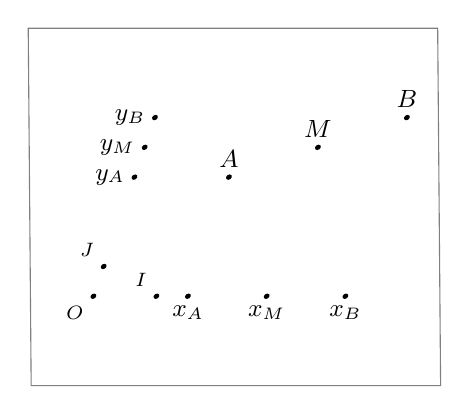
\begin{tikzpicture}[scale=0.40]
		\tkzInit[xmin=-8,xmax=10,ymin=-7,ymax=8  ]
		\pgftransformcm{1}{0}{sin(19)}{cos(19)}{\pgfpointorigin}
		\path[clip,preaction = {draw=gray}] 
		(+12,-3) -- (-1,-3) -- (-5,9) -- (8,9) -- cycle;
		%\tkzGrid[color=gray](-9,-7)(11,7)
		\tkzDrawXY[ noticks, line width=1pt] 
		\filldraw 
		(0,0) circle (2pt) node[align=left, below left] {\scriptsize $O$} ;
		\filldraw 
		(2,0) circle (2pt) node[align=left, above left] {\scriptsize $I$} ;
		\filldraw 
		(0,1) circle (2pt) node[align=left, above left] {\scriptsize$J$} ;
		\filldraw 
		(3,4) circle (2pt) node[align=left, above] {\small$A$} ;
		\filldraw 
		(3,0) circle (2pt) node[align=left, below] {\small$x_A$} ;
		\filldraw 
		(0,4) circle (2pt) node[align=left, left] {\small$y_A$} ;
		\filldraw  
		(8,6) circle (2pt) node[align=left, above] {\small$B$} ;
		\filldraw 
		(8,0) circle (2pt) node[align=left, below] {\small$x_B$} ;
		\filldraw 
		(0,6) circle (2pt) node[align=left, left] {\small$y_B$} ;
		\filldraw  
		(5.5,5) circle (2pt) node[align=left, above] {\small$M$} ;
		\filldraw 
		(5.5,0) circle (2pt) node[align=left, below] {\small$x_M$} ;
		\filldraw 
		(0,5) circle (2pt) node[align=left, left] {\small$y_M$} ;
		\filldraw 	;		
		\tkzDefPoint(5.5, 5){M};
		\tkzDefPoint(5.5,0){xM};
		\tkzDefPoint(0, 5){yM};
		\tkzDrawSegments[dashed](M,xM M,yM);
		\tkzDefPoint(3,4){A};
		\tkzDefPoint(3,0){xA};
		\tkzDefPoint(0,4){yA};
		\tkzDrawSegments[dashed](A,xA A,yA);
		\tkzDefPoint(8,6){B};
		\tkzDefPoint(8,0){xB};
		\tkzDefPoint(0,6){yB};
		\tkzDrawSegments[dashed](B,xB B,yB);
		\tkzDrawSegments[line width=2pt](A,M M,B);
		\tkzMarkSegments[mark=s||](A,M M,B);
		\tkzMarkSegments[mark=|||](xA,xM xM,xB);
		\tkzMarkSegments[mark=s|](yA,yM yM,yB);
	\end{tikzpicture}  
\end{marginfigure} 
\begin{proof}[Démonstration]\hfill 
	\begin{align*}
		&\text{$M$ est le milieu de $[AB]$} \\
		& \iff \vv{AM}=\vv{MB} \\
		& \iff \vv{AM}\begin{pmatrix}
			x_M-x_A \\ y_M-y_A
		\end{pmatrix}=\vv{MB}\begin{pmatrix}
			x_B-x_M\\ y_B-y_M
		\end{pmatrix} \\
		& \iff \begin{cases}
			x_M-x_A = x_B-x_M  \\  y_M-y_A = y_B-y_M
		\end{cases} 
		\iff \begin{cases}
			2x_M = x_A + x_B  \\ 2y_M = y_A + y_B
		\end{cases} \\
		& \iff \begin{cases}
			x_M =\frac{x_A+x_B}{2} \\ y_M =\frac{y_A+y_B}{2}
		\end{cases}  
	\end{align*} 
	%	\vfill 
\end{proof} 
\begin{theorem}[formule pour les coordonnées du milieu d'un segment]
	Soit $A(x_A;y_A)$ et $B(x_B;y_B)$ dans un repère.
	
	Le milieu $M(x_M;y_M)$ de $[AB]$ est le point de coordonnées :
	\begin{align*}
		x_M&=\frac{x_A+x_B}{2}\\
		y_M&=\frac{y_A+y_B}{2}
	\end{align*}
\end{theorem} 


\begin{example}
	On considère les points $A(1~;~2)$, $B(3~;~1,5)$, $C(4~;~0,5)$ et $D(2~;~1)$.  
	Montrer que le quadrilatère $ABCD$ est un parallélogramme en déterminant les coordonnées des milieux des diagonales.
\end{example}
\vfill 


%----------------------------------------------------------------------------------------
%	 
%----------------------------------------------------------------------------------------



%----------------------------------------------------------------------------------------
%	 
%----------------------------------------------------------------------------------------


\newpage 
\loadgeometry{widelayout}  
\pagestyle{scrheadings} % Print headers again  
\KOMAoptions{
	headwidth=textwithmarginpar,
	headsepline=true,
	headsepline= 0.5pt,
	footwidth=textwithmarginpar,
} 
\onehalfspacing
\subsection{Exercices égalités vectorielles}

%----------------------------------------------------------------------------------------
%	 
%----------------------------------------------------------------------------------------


\begin{exercise}[Égalités vectorielles]\label{chapter06:exercices:egalitesvectoriels} À l'aide d'un schéma, préciser les énoncés vrais.\hfill     
	
	\noindent\QCM[VF,Alterne,Largeur=1.0cm,Stretch=1.1]{%
		{$Q$ est l'image de $P$ par la translation $\vv{AB}$, alors $\vv{PQ}=\vv{AB}$}&1,% 
		{$Q$ est l'image de $P$ par la translation $\vv{AB}$, alors $\vv{AP}=\vv{BQ}$}&2,% 
		{Le quadrilatère $JOLI$ est un parallélogramme revient à dire $\vv{JO}=\vv{LI}$}&2,% 
		{Le quadrilatère $JOLI$ est un parallélogramme revient à dire $\vv{OJ}=\vv{LI}$}&1,% 
		{Le quadrilatère $JOLI$ est un parallélogramme revient à dire $\vv{OL}=\vv{JI}$}&1,% 
		{Le quadrilatère $JOLI$ est un parallélogramme revient à dire $\vv{OL}=\vv{IJ}$}&2,%
		{Si $I$ est le centre du parallélogramme $ECHO$ alors $\vv{EI}=\vv{IC}$}&2,%   
		{Si $I$ est le centre du parallélogramme $ECHO$ alors $\vv{IO}=\vv{CI}$}&1,%   
		{Si $Q$ est l'image de $P$ par la symétrie de centre $R$, alors $\vv{PR}=\vv{RQ}$}&1,% 
		{Si $M$ est le milieu de $[AB]$ alors $AM=BM$}&2,% 
		{Si $AM=BM$ alors $M$ est nécessairement le milieu de $[AB]$}&2,% 
		{Si $\vv{AM}=\vv{MB}$ alors $M$ est nécessairement le milieu de $[AB]$}&2,%
		{Si $\vv{AB}=\vv{DC}$ alors  $AB=CD$}&1,%
		{Si $AB=CD$ alors  $\vv{AB}=\vv{DC}$}&2,%
		{Si $\vv{AB}=\vv{DC}$ alors $\vv{BC}=\vv{AD}$}&1,% 
	} 
\end{exercise}
%----------------------------------------------------------------------------------------
%	 
%----------------------------------------------------------------------------------------


\begin{example}[je fais]\hfill
	
	Dans un repère on donne les points : $I(2 ; -2)$, $J(-1 ; -1)$, $K(0 ; 1)$, $L(-3 ; 2)$. 
	\begin{enumerate}[leftmargin=*,label=\alph*)] 
		\item Montrer par le calcul que $IJLK$ est un parallélogramme.
		\vfill 
		\item Trouver par le calcul le point $M(x;y)$ tel que $ILMJ$ est un parallélogramme.
		\vfill 
	\end{enumerate} 
\end{example}

\begin{exercise} \label{chapter06:exercices:parallelogrammes01}
	Soit les points $A(-3~;~-1)$, $B(5~;~-2)$, $C(7~;~3)$ et $D(-1~;~4)$ dans le repère $(O;I,J)$. 
	
	Montrer que  $ABCD$  est un parallélogramme.
\end{exercise}

\begin{exercise} \label{chapter06:exercices:parallelogrammes02}
	Soit les points $A(11,-14)$, $B(-13,12)$ et $C(-4,7)$ dans le repère $(O;I,J)$.
	
	Trouver les coordonnées de $M(x;y)$ tel que $ABMC$ est un parallélogramme.
\end{exercise}
%----------------------------------------------------------------------------------------
%	 
%----------------------------------------------------------------------------------------

\newpage
\begin{exercise} \label{chapter06:exercices:parallelogrammes03}
	Soit les points $A(12~;~15)$, $B(-11~;~17)$ et $C(-11~;~-13)$. 
	
	Calculer les coordonnées du point $D(x;y)$ tel que $ABCD$ soit un parallélogramme.
\end{exercise}  
\begin{exercise}\label{chapter06:exercices:parallelogrammes04} Soit les points   $D(-14;15)$; $A(16;11)$; $T(15;-7)$. 
	
	$DARK$ est le parallélogramme de centre $T$ (intersection des diagonales). Retrouver par le calcul les coordonnées de $R$ et $K$. 
\end{exercise}
\begin{exercise}[Variations]\label{chapter06:exercices:parallelogrammes05} 
	Le plan est muni d'un repère $(O;I,J)$.  Pour chacun des cas suivants, traduire la propriété donnée en une égalité de vecteurs. En déduire les équations vérifiées par les coordonnées de $M(x;y)$, et les résoudre.
	\begin{enumerate}[label=\alph*)]
		\item $A(-1;1)$, $B = ( -1; 2)$. $M(x;y)$ est tel que $ABMO$ est un parallélogramme.
		\item  $A( -1; 2)$, $B = (3; 1)$.  $M(x;y)$ est tel que $AMBO$ est un parallélogramme.
		\item  $A(-2;1)$, $B = (1;2)$.  $M(x;y)$ est tel que $ABMI$ est un parallélogramme.
		\item $A(-3;-2)$, $B(-1;-1)$. $M(x;y)$ est tel que $A$ est le milieu du segment $[MB]$
		\item $A(-3;-2)$, $B(-1;-1)$. $M(x;y)$ est tel que $M$ est le milieu du segment $[AB]$ 
		\item $A(2;5)$, $B = (1; 1)$. $M(x;y)$ est tel que $M$ est le milieu du segment $[AB]$ 
		\item $A(1;5)$. $M(x;y)$ est le symétrique de $A$ par rapport à l'origine $O$.
	\end{enumerate}
\end{exercise}  
\begin{eBox}
	Dans les exercices suivants, le repère $(O;I,J)$ est orthonormé.
\end{eBox} 
\begin{exercise} Soit les points $B(-10;-5)$ , $E(-16;3)$, $A(-48;-21)$ et $U(-42;-29)$
	\begin{enumerate}[label=\alph*), leftmargin=*]\label{chapter06:exercice:naturequadrilatere01}
		\item Montrer que $BEAU$ est un parallélgoramme.
		\item Calculer les longueurs des côtés adjacents $BE$ et $EA$.
		\item Calculer les longueurs des diagonales $BA$ et $EU$. 
		\item Que pouvez vous dire du quadrilatère $BEAU$ ?
	\end{enumerate}
\end{exercise}
\begin{exercise}\label{chapter06:exercice:naturequadrilatere02} Soit les points $C(-7;9)$ , $A(\numprint{6.5};2)$, $F(-4;13)$ et $E(-\numprint{17.5};20)$
	\begin{enumerate}[label=\alph*), leftmargin=*]
		\item Montrer que $CAFE$ est un parallélgoramme.
		\item Calculer les longueurs des diagonales $CF$ et $AE$.
		\item Calculer les longueurs des côtés adjacents $CA$ et $AF$.
		\item  Que pouvez vous dire du quadrilatère $CAFE$ ?
	\end{enumerate}
\end{exercise} 
\begin{exercise} Soit le parallélogramme $ARMY$ tel que $A(-6;7)$; $R(-11;9)$; $Y(-7;13)$.\hfill 
	\begin{enumerate}[label=\alph*), leftmargin=*]
		\item Calculer la longueur de la diagonale $RY$  
		\item Calculer les coordonnées de $M$, et en déduire la longueur de la diagone $AM$.
	\end{enumerate}
\end{exercise} 
\begin{eBox}
	Dans les 2 derniers exercices, utiliser directement la formule des coordonnées du milieu d'un segment sans passez par des égalités vectorielles.
\end{eBox} 
\begin{exercise}  Soit $F(10;−8)$, $U(13;0)$, $N(24;9)$ et $F(21;1)$.
	
	Montrer que $FUNK$ est un parallélogramme en démontrant que les diagonales ont même milieu. 
\end{exercise}
\begin{exercise} 	Soit $P(2;3)$, $Q(5;4)$ et $R(4;5)$. 
	\begin{enumerate}[label=\alph*)]
		\item Calculer les coordonnées du milieu de $[PQ]$.
		\item Montrer que $R$ appartient au cercle de diamètre $[PQ]$.
	\end{enumerate} 
\end{exercise}  


%----------------------------------------------------------------------------------------
%	 
%----------------------------------------------------------------------------------------


\newpage 

\begin{proof}[solution de l'exercice \ref{chapter06:exercice:vecteur:coordonneesgraphique}]\hfill 
	
	\noindent	$\vv{AA'}\begin{pmatrix}
		2 \\ 2
	\end{pmatrix}$, $\vv{BB'}\begin{pmatrix}
		3 \\ -1
	\end{pmatrix}$, $\vv{CC'}\begin{pmatrix}
		7 \\ -3
	\end{pmatrix}$, $\vv{DD'}\begin{pmatrix}
		-2 \\ 4
	\end{pmatrix}$, $\vv{EE'}\begin{pmatrix}
		6 \\ 1
	\end{pmatrix}$
	
	\noindent	\begin{minipage}{1\columnwidth}\centering
		\begin{tikzpicture}[scale=0.70 			]
			\tkzSetUpPoint[size=3, fill=black]
			\tkzfctset{tan style/.style={->,>=latex, color=red, line width=1.2pt}}   
			\tkzSetUpLine[line width= 1.2pt, add=.5 and .5] 
			
			
			\tkzInit[xmin=-8, ymin=-6,  xmax=15,ymax=12]  
			\begin{scope}[dashed] 
				\tkzGrid 
			\end{scope}  
			\tkzDrawX[ above=5pt,  label=$x$, font=\scriptsize, line width=1.2pt ] %, style=dashed
			\tkzDrawY[ right =5pt, label=$y$, font=\scriptsize, line width=1.2pt]  %, style=dashed
			\tkzRep[color  = Maroon,line width = 2pt, posxlabel=below, posylabel=left, xnorm=1,ynorm=1, xlabel={}, ylabel={}] 
			
			
			
			\tkzDefPoint(7,-4){A} 
			\tkzDefShiftPoint[A](2,2){A'} 
			\tkzDrawSegment[->,>=latex, line width=1.2](A,A') 
			\tkzLabelSegment[above left](A,A') {\scriptsize $\vv{AA'}$}
			\tkzLabelPoint[below](A){\scriptsize$A$}\tkzLabelPoint[right](A'){\scriptsize$A'$}
			
			\tkzDefPoint(1,-2){B} 
			\tkzDefShiftPoint[B](3,-1){B'} 
			\tkzDrawSegment[->,>=latex, line width=1.2](B,B') 
			\tkzLabelSegment[above](B,B') {\scriptsize $\vv{BB'}$}
			\tkzLabelPoint[below](B){\scriptsize$B$}\tkzLabelPoint[right](B'){\scriptsize$B'$}
			
			\tkzDefPoint(-7,8){C} 
			\tkzDefShiftPoint[C](7,-3){C'} 
			\tkzDrawSegment[->,>=latex, line width=1.2](C,C') 
			\tkzLabelSegment[above](C,C') {\scriptsize $\vv{CC'}$}
			\tkzLabelPoint[below](C){\scriptsize$C$}\tkzLabelPoint[right](C'){\scriptsize$C'$}
			
			\tkzDefPoint(6,8){D} 
			\tkzDefShiftPoint[D](-2,4){D'} 
			\tkzDrawSegment[->,>=latex, line width=1.2](D,D') 
			\tkzLabelSegment[right](D,D') {\scriptsize $\vv{DD'}$}
			\tkzLabelPoint[below](D){\scriptsize$D$}\tkzLabelPoint[right](D'){\scriptsize$D'$}
			
			\tkzDefPoint(8,10){E} 
			\tkzDefShiftPoint[E](6,1){E'} 
			\tkzDrawSegment[->,>=latex, line width=1.2](E,E') 
			\tkzLabelSegment[above](E,E') {\scriptsize $\vv{EE'}$}
			\tkzLabelPoint[below](E){\scriptsize$E$}\tkzLabelPoint[right](E'){\scriptsize$E'$}
			
			
			
			
			\tkzDefPoint(2,5){M}
			\tkzDefPoint(3,1){N}
			\tkzDefPoint(7,6){P} 
			\tkzDefShiftPoint[M](2,2){M1}
			\tkzDrawSegment[->,>=latex, line width=1.2,blue](M,M1) 
			\tkzLabelPoint[right](M1){$M'$}
			
			\tkzDefShiftPoint[N](3,-1){N1}
			\tkzDrawSegment[->,>=latex, line width=1.2,blue](N,N1) 
			\tkzLabelPoint[right](N1){$N'$}
			
			\tkzDefShiftPoint[P](-7,+3){P1}
			\tkzDrawSegment[->,>=latex, line width=1.2,blue](P1,P) 
			\tkzLabelPoint[right](P1){$P'$}
			
			
			\tkzDefPoint(11,2){Q} 
			\tkzDrawPoint(Q)\tkzLabelPoint[above right](Q){$Q$}
			\tkzDefShiftPoint[Q](2,-4){Q1}
			\tkzDrawSegment[->,>=latex, line width=1.2,blue](Q1,Q) 
			\tkzLabelPoint[right](Q1){$Q'$}
			
			
			\tkzDefShiftPoint[E](0,2){S}
			\tkzDrawSegment[->,>=latex, line width=1.2,red](E,S) 
			\tkzDrawPoint(S)\tkzLabelPoint[above right](S){$S$}
			
			\tkzDefShiftPoint[A](4,0){T}
			\tkzDrawSegment[->,>=latex, line width=1.2,red](A,T) 
			\tkzDrawPoint(T)\tkzLabelPoint[above right](T){$T$}
			
			\tkzDefShiftPoint[B](4,3){U}
			\tkzDrawSegment[->,>=latex, line width=1.2,red](B,U) 
			\tkzDrawPoint(U)\tkzLabelPoint[above right](U){$U$}
			
			\tkzDefPoint(0,0){O}	
			\tkzDefShiftPoint[O](-4,-3){V}
			\tkzDrawSegment[->,>=latex, line width=1.2,red](O,V) 
			\tkzDrawPoint(V)\tkzLabelPoint[above left](V){$V$}
			
			
			\tkzDefShiftPoint[O](+6,1){R}
			\tkzDrawSegment[->,>=latex, line width=1.2,blue](O,R) 
			\tkzDrawPoint(R)\tkzLabelPoint[above left](R){$R$}
			
			
			\tkzDefShiftPoint[D](-4,+2){W}
			\tkzDrawSegment[->,>=latex, line width=1.2,red](W,D) 
			\tkzDrawPoint(W)\tkzLabelPoint[above left](W){$W$}
			
			
			\tkzDefShiftPoint[E](+3,-5){X}
			\tkzDrawSegment[->,>=latex, line width=1.2,red](X,E) 
			\tkzDrawPoint(X)\tkzLabelPoint[above left](X){$X$}
			
			
			
			%		\tkzDefShiftPoint[M](3,-1){M2}
			%		\tkzDefShiftPoint[M](7,-3){N1} 
			%		  	  	\tkzDrawSegment[->,>=latex, line width=1.2](M1,P) 
			%		  	  	\tkzDrawSegment[->,>=latex, line width=1.2](M,M2) 
			%		  	  	\tkzDrawSegment[->,>=latex, line width=1.2](M2,P) 
			%			  	\tkzDrawSegment[->,>=latex, line width=1.2](M,N1) 
			%			  	\tkzDrawSegment[->,>=latex, line width=1.2](N1,P) 
			%			  	\tkzDrawSegment[->,>=latex, line width=1.2](N,N1) 
			%		  	\tkzLabelSegment[above](M,M1){\small $\vv{a}$}
			%			  	\tkzLabelSegment[above](M1,P) {\small $\vv{b}$}
			%			  	\tkzLabelSegment[above](M,M2){\small $\vv{b}$}
			%			  	\tkzLabelSegment[above](M2,P) {\small $\vv{a}$}
			%		%	  	\tkzLabelSegment[below](M,N1)  {\small $\vv{c}$}
			%			  	\tkzLabelSegment[right](N1,P)  {\small $\vv{d}$}
			%			  	\tkzLabelSegment[above](N,N1)   {\small $\vv{e}$} 	  	  	
			
			
			
			\tkzDrawPoints[color=black, size=2](M,N,P)
			\tkzLabelPoint[above](M){\scriptsize$M$} 
			\tkzLabelPoint[below](N){\scriptsize$N$}  
			\tkzLabelPoint[above right](P){\scriptsize$P$} 
			\filldraw 
			(0,0) circle (2pt) node[align=left, below left] {\scriptsize $O$} ;
			\filldraw 
			(1,0) circle (2pt) node[align=left, below] {\scriptsize $I$} ;
			\filldraw 
			(0,1) circle (2pt) node[align=left, left] {\scriptsize $J$} ; 
		\end{tikzpicture} 
	\end{minipage} 
\end{proof}

\begin{multicols}{2}  
	\begin{proof}[solution de l'exercice \ref{chapter06:exercice:vecteurscoordonnees}]\hfill 
		\begin{enumerate}[leftmargin=*,label=\alph*)] 
			\item  $\vv{AB}\begin{pmatrix}
				-11\\-1
			\end{pmatrix}$;
			$\vv{BC}\begin{pmatrix}
				8\\17
			\end{pmatrix}$;
			$\vv{CA}\begin{pmatrix}
				3\\-16
			\end{pmatrix}$;
			\item  $\vv{AB}\begin{pmatrix}
				5\\-5
			\end{pmatrix}$;
			$\vv{BC}\begin{pmatrix}
				1\\2
			\end{pmatrix}$;
			$\vv{CA}\begin{pmatrix}
				-6\\3
			\end{pmatrix}$;
			\item  $\vv{AB}\begin{pmatrix}
				-4\\5
			\end{pmatrix}$;
			$\vv{BC}\begin{pmatrix}
				7\\\sqrt{2}-5
			\end{pmatrix}$;
			$\vv{CA}\begin{pmatrix}
				-3\\-\sqrt{2}
			\end{pmatrix}$;
			\item  $\vv{AB}\begin{pmatrix}
				-5\\-3
			\end{pmatrix}$;
			$\vv{BC}\begin{pmatrix}
				7\\-2
			\end{pmatrix}$;
			$\vv{CA}\begin{pmatrix}
				-2\\5 
			\end{pmatrix}$;
		\end{enumerate} 
	\end{proof}
	\begin{proof}[solution de l'exercice \ref{chapter06:exercice:translationcoordonnees}]\hfill 
		\begin{enumerate}[leftmargin=*,label=\alph*)] 
			\item  $\vv{AB}\begin{pmatrix}
				-4\\-1
			\end{pmatrix}$ et $M(-4;-1)$.
			\item  $\vv{BC}\begin{pmatrix}
				-4\\-4
			\end{pmatrix}$ et $M(-3;-7)$.
			\item  $\vv{CA}\begin{pmatrix}
				8\\5
			\end{pmatrix}$; $I(1;0)$ et $M(9;5)$.
			\item $\vv{CA}\begin{pmatrix}
				8\\5
			\end{pmatrix}$; $J(0;1)$ et $M(-8;-4)$.
		\end{enumerate} 
	\end{proof} 
\end{multicols}

\begin{proof}[solution de l'exercice \ref{chapter06:exercices:egalitesvectoriels}] \hfill 
	
	\noindent\QCM[VF,Alterne,Largeur=1.0cm,Stretch=1.1, Solution ]{%
		{$Q$ est l'image de $P$ par la translation $\vv{AB}$, alors $\vv{PQ}=\vv{AB}$}&1,% 
		{$Q$ est l'image de $P$ par la translation $\vv{AB}$, alors $\vv{AP}=\vv{BQ}$}&2,% 
		{Le quadrilatère $JOLI$ est un parallélogramme revient à dire $\vv{JO}=\vv{LI}$}&2,% 
		{Le quadrilatère $JOLI$ est un parallélogramme revient à dire $\vv{OJ}=\vv{LI}$}&1,% 
		{Le quadrilatère $JOLI$ est un parallélogramme revient à dire $\vv{OL}=\vv{JI}$}&1,% 
		{Le quadrilatère $JOLI$ est un parallélogramme revient à dire $\vv{OL}=\vv{IJ}$}&2,%
		{Si $I$ est le centre du parallélogramme $ECHO$ alors $\vv{EI}=\vv{IC}$}&2,%   
		{Si $I$ est le centre du parallélogramme $ECHO$ alors $\vv{IO}=\vv{CI}$}&1,%   
		{Si $Q$ est l'image de $P$ par la symétrie de centre $R$, alors $\vv{PR}=\vv{RQ}$}&1,% 
		{Si $M$ est le milieu de $[AB]$ alors $AM=BM$}&2,% 
		{Si $AM=BM$ alors $M$ est nécessairement le milieu de $[AB]$}&2,% 
		{Si $\vv{AM}=\vv{MB}$ alors $M$ est nécessairement le milieu de $[AB]$}&2,%
		{Si $\vv{AB}=\vv{DC}$ alors  $AB=CD$}&1,%
		{Si $AB=CD$ alors  $\vv{AB}=\vv{DC}$}&2,%
		{Si $\vv{AB}=\vv{DC}$ alors $\vv{BC}=\vv{AD}$}&1,% 
	} 
\end{proof}
\begin{proof}[solution de l'exercice  \ref{chapter06:exercices:parallelogrammes01}]   
	
	$\vv{AB}\begin{pmatrix}
		8\\ -1
	\end{pmatrix} =\vv{DC}\begin{pmatrix}
		8\\ -1
	\end{pmatrix}$.
\end{proof}
\begin{proof}[solution de l'exercice \ref{chapter06:exercices:parallelogrammes02}]   
	
	$\vv{AB}\begin{pmatrix}
		-24\\ 26
	\end{pmatrix} =\vv{DC}\begin{pmatrix}
		x+4\\ y-7
	\end{pmatrix}$. $M(-28;33)$.
\end{proof}
\begin{proof}[solution de l'exercice  \ref{chapter06:exercices:parallelogrammes03}]   
	
	$\vv{AB}\begin{pmatrix}
		-23\\ 2 
	\end{pmatrix} =\vv{DC}\begin{pmatrix}
		-11-x\\ -13-y
	\end{pmatrix}$. $M(12;-15)$.
\end{proof}
\begin{proof}[solution de l'exercice  \ref{chapter06:exercices:parallelogrammes04}]   
	
	$\vv{DT}\begin{pmatrix}
		29\\ -22 
	\end{pmatrix} =\vv{TR}\begin{pmatrix}
		x-15\\ y+7
	\end{pmatrix}$. $R(44;-29)$.
	
	$\vv{AT}\begin{pmatrix}
		-1\\ -18 
	\end{pmatrix} =\vv{TK}\begin{pmatrix}
		x-15\\ y+7
	\end{pmatrix}$. $K(14;-25)$.
\end{proof}
\begin{proof}[solution de l'exercice  \ref{chapter06:exercices:parallelogrammes05}]   
	\begin{enumerate}[label=\alph*)]
		\item $\vv{OM}\begin{pmatrix}
			x\\ y 
		\end{pmatrix} =\vv{TR}\begin{pmatrix}
			0\\ 1
		\end{pmatrix}$. $M(0;1)$.
		\item $\vv{OA}\begin{pmatrix}
			-1\\ 2 
		\end{pmatrix} =\vv{BM}\begin{pmatrix}
			x-3\\ y-1
		\end{pmatrix}$. $M(2;3)$.
		\item $\vv{AB}\begin{pmatrix}
			3\\ 1 
		\end{pmatrix} =\vv{IM}\begin{pmatrix}
			x-1\\ y-0
		\end{pmatrix}$. $M(4;1)$.
		\item $\vv{BA}\begin{pmatrix}
			-2\\ -1 
		\end{pmatrix} =\vv{AM}\begin{pmatrix}
			x+3\\ y+2
		\end{pmatrix}$. $M(-5;-3)$.
		\item $\vv{AM}\begin{pmatrix}
			x+3\\ y+2 
		\end{pmatrix} =\vv{MB}\begin{pmatrix}
			-1-x\\ -1-y
		\end{pmatrix}$. $M(-2;-\tfrac{3}{2})$.
		\item $\vv{AM}\begin{pmatrix}
			x-2\\ y-5 
		\end{pmatrix} =\vv{MB}\begin{pmatrix}
			1-x\\ 1-y
		\end{pmatrix}$. $M(\tfrac{3}{2};3)$.
		\item $\vv{AO}\begin{pmatrix}
			-1\\ -5 
		\end{pmatrix} =\vv{OM}\begin{pmatrix}
			x\\ y
		\end{pmatrix}$. $M(-1;-5)$.
	\end{enumerate} 
\end{proof}
\begin{proof}[solution de l'exercice  \ref{chapter06:exercice:naturequadrilatere01}]   \hfill
	
	\begin{enumerate}[label=\alph*)]
		\item $\vv{BE}\begin{pmatrix}
			-6\\ 8 
		\end{pmatrix} =\vv{UA}\begin{pmatrix}
			-6\\ 8
		\end{pmatrix}$
		\item  $BE=10$  et $EA =40$.
		\item $BA=10\sqrt{17}$ et $EU=10\sqrt{17}$.
		\item $BEAU$ est un rectangle qui n'est pas carré.
	\end{enumerate} 
\end{proof}
\begin{proof}[solution de l'exercice  \ref{chapter06:exercice:naturequadrilatere02}]  \hfill  
	
	\begin{enumerate}[label=\alph*)]
		\item $\vv{CA}\begin{pmatrix}
			\numprint{13.5}\\ -7 
		\end{pmatrix} =\vv{UA}\begin{pmatrix}
			\numprint{13.5}\\ -7 
		\end{pmatrix}$
		\item $CA=AF=\tfrac{5\sqrt{37}}{2}$.
		\item $CF=5$ et $AE=\sqrt{445}$.
		\item $CAFE$ est un losange qui n'est pas carré.
	\end{enumerate} 
\end{proof}

 

%----------------------------------------------------------------------------------------
%	 
%----------------------------------------------------------------------------------------
\end{document}